\documentclass[a4paper, 11pt]{article}
\usepackage{graphicx}
\usepackage{multicol}
\usepackage{tabularx}
\usepackage{enumitem}
\usepackage[a4paper, margin=1.8cm]{geometry}
\usepackage{listings}
\usepackage{amssymb}
\usepackage{gvv}
\usepackage{gvv-book}
\usepackage{amsmath}
\usepackage{setspace}
\usepackage{caption}
\usepackage{tfrupee}
\usepackage{float}
\usepackage{quoting}

\graphicspath{ {./figs} }

\begin{document}
\begin{center}
    \huge{CS: COMPUTER SCIENCE AND INFORMATION TECHNOLOGY-2025}\\
    \large{EE25BTECH11041 - Naman Kumar}
\end{center}


\begin{enumerate}
    \item Ravi had \underline{\hspace{2cm}} younger brother who taught at \underline{\hspace{2cm}} university. He was widely regarded as \underline{\hspace{2cm}} honorable man.\\Select the option with the correct sequence of articles to fill in the blanks.
    \begin{enumerate}
        \begin{multicols}{4}
            \item a; a; an
            \item the; an; a
            \item a; an; a
            \item an; an; a
        \end{multicols}
    \end{enumerate}
    \hfill{\brak{\text{GATE CS 2025}}}
    \item The CEO's decision to downsize the workforce was considered myopic because it sacrificed long-term stability to accommodate short-term gains.\\Select the most appropriate option that can replace the word "myopic" without changing the meaning of the sentence.
    \begin{enumerate}
        \begin{multicols}{4}
            \item visionary
            \item shortsighted
            \item progressive
            \item innovative
        \end{multicols}
    \end{enumerate}
    \hfill{\brak{\text{GATE CS 2025}}}
    \item The average marks obtained by a class in an examination were calculated as $30.8$. However, while checking the marks entered, the teacher found that the marks of one student were entered incorrectly as $24$ instead of $42$. After correcting the marks, the average becomes $31.4$. How many students does the class have?
    \begin{enumerate}
        \begin{multicols}{4}
            \item $25$
            \item $28$
            \item $30$
            \item $32$
        \end{multicols}
    \end{enumerate}
    \hfill{\brak{\text{GATE CS 2025}}}
    \item Consider the relationships among P, Q, R, S, and T:
    \begin{itemize}
        \item P is the brother of Q.
        \item S is the daughter of Q.
        \item T is the sister of S.
        \item R is the mother of Q.
    \end{itemize}
    The following statements are made based on the relationships given above.
    \begin{enumerate}[label=\brak{\arabic*}]
        \item R is the grandmother of S.
        \item P is the uncle of S and T.
        \item R has only one son.
        \item Q has only one daughter.
    \end{enumerate}
    Which one of the following options is correct?
    \begin{enumerate}
        \item Both \brak{1} and \brak{2} are true.
        \item Both \brak{1} and \brak{3} are true.
        \item Only \brak{3} is true.
        \item Only \brak{4} is true.
    \end{enumerate}
    \hfill{\brak{\text{GATE CS 2025}}}
    \item According to the map shown in the figure, which one of the following statements is correct?\\Note: The figure shown is representative.
    \begin{figure}[H]
        \centering
        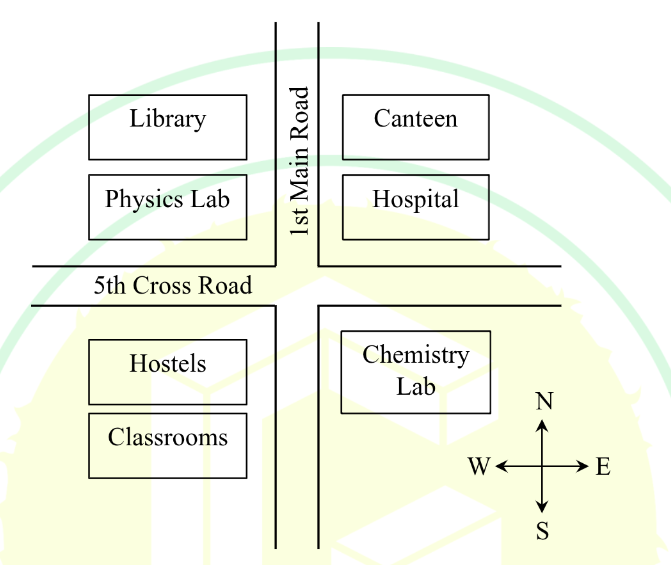
\includegraphics[width=0.6\columnwidth]{figs/q5.png}
        \label{fig:placeholder}
    \end{figure}
    \begin{enumerate}
        \item The library is located to the northwest of the canteen.
        \item The hospital is located to the east of the chemistry lab.
        \item The chemistry lab is to the southeast of physics lab.
        \item The classrooms and canteen are next to each other.
    \end{enumerate}
    \hfill{\brak{\text{GATE CS 2025}}}
    \item 
    \begin{quoting}
    "I put the brown paper in my pocket along with the chalks, and possibly other things. I suppose every one must have reflected how primeval and how poetical are the things that one carries in one's pocket: the pocket-knife, for instance the type of all human tools, the infant of the sword. Once I planned to write a book of poems entirely about the things in my pocket. But I found it would be too long: and the age of the great epics is past."\\
    \brak{\text{From G.K. Chesterton's "A Piece of Chalk"}}
    \end{quoting}
    Based only on the information provided in the above passage, which one of the following statements is true?
    \begin{enumerate}
        \item The author of the passage carries a mirror in his pocket to reflect upon things.
        \item The author of the passage had decided to write a poem on epics.
        \item The pocket-knife is described as the infant of the sword.
        \item Epics are described as too inconvenient to write.
    \end{enumerate}
    \hfill{\brak{\text{GATE CS 2025}}}
    \item In the diagram, the lines QR and ST are parallel to each other. The shortest distance between these two lines is half the shortest distance between the point P and line QR. What is the ratio of the area of the triangle PST to the area of the trapezium SQRT?\\Note: The figure shown is representative.
    \begin{figure}[H]
        \centering
        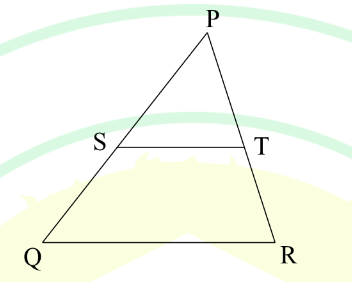
\includegraphics[width=0.4\columnwidth]{figs/q7.png}
        \label{fig:placeholder}
    \end{figure}
    \begin{enumerate}
        \begin{multicols}{4}
            \item $\frac{1}{3}$
            \item $\frac{1}{4}$
            \item $\frac{2}{5}$
            \item $\frac{1}{2}$
        \end{multicols}
    \end{enumerate}
    \hfill{\brak{\text{GATE CS 2025}}}
    \item A fair six-faced dice, with the faces labelled '1', '2', '3', '4', '5', and '6', is rolled thrice. What is the probability of rolling '6' exactly once?
    \begin{enumerate}
        \begin{multicols}{4}
            \item $\frac{75}{216}$
            \item $\frac{1}{6}$
            \item $\frac{1}{18}$
            \item $\frac{25}{216}$
        \end{multicols}
    \end{enumerate}
    \hfill{\brak{\text{GATE CS 2025}}}
    \item A square paper, shown in figure \brak{I}, is folded along the dotted lines as shown in the figures \brak{II} and \brak{III}. Then a few cuts are made as shown in figure \brak{IV}. Which one of the following patterns will be obtained when the paper is unfolded?\\Note: The figures shown are representative.
    \begin{figure}[H]
        \centering
        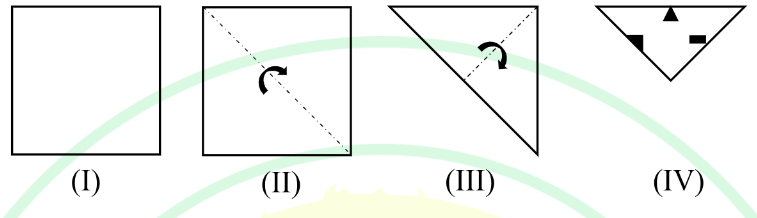
\includegraphics[width=0.8\columnwidth]{figs/q9.png}
        \caption*{}
        \label{fig:q9}
    \end{figure}
    \begin{enumerate}
        \item 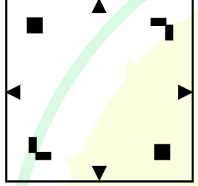
\includegraphics[width=0.2\columnwidth]{figs/q9A.png}
        \item 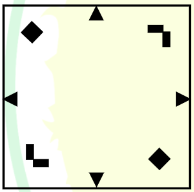
\includegraphics[width=0.2\columnwidth]{figs/q9B.png}
        \item 
\includegraphics[width=0.2\columnwidth]{figs/q9C.png}
        \item 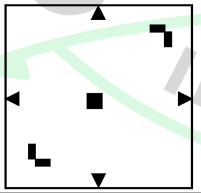
\includegraphics[width=0.2\columnwidth]{figs/q9D.png}
    \end{enumerate}
    \hfill{\brak{\text{GATE CS 2025}}}
    \item A shop has $4$ distinct flavors of ice-cream. One can purchase any number of scoops of any flavor.\textbf{The order in which the scoops are purchased is inconsequential.} If one wants to purchase $3$ scoops of ice-cream, in how many ways can one make that purchase?
    \begin{enumerate}
        \begin{multicols}{4}
            \item $4$
            \item $20$
            \item $24$
            \item $48$
        \end{multicols}
    \end{enumerate}
    \hfill{\brak{\text{GATE CS 2025}}}
    \item Suppose a program is running on a non-pipelined single processor computer system. The computer is connected to an external device that can interrupt the processor asynchronously. The processor needs to execute the interrupt service routine \brak{ISR} to serve this interrupt. The following steps \brak{not necessarily in order} are taken by the processor when the interrupt arrives:
    \begin{enumerate}[label=\brak{\roman*}]
        \item The processor saves the content of the program counter.
        \item The program counter is loaded with the start address of the ISR.
        \item The processor finishes the present instruction.
    \end{enumerate}
    Which ONE of the following is the CORRECT sequence of steps?
    \begin{enumerate}
        \begin{multicols}{2}
            \item \brak{iii}, \brak{i}, \brak{ii}
            \item \brak{i}, \brak{iii}, \brak{ii}
            \item \brak{i}, \brak{ii}, \brak{iii}
            \item \brak{iii}, \brak{ii}, \brak{i}
        \end{multicols}
    \end{enumerate}
    \hfill{\brak{\text{GATE CS 2025}}}
    \item Which ONE of the following statements is \textbf{FALSE} regarding the symbol table?
    \begin{enumerate}
        \item Symbol table is responsible for keeping track of the scope of variables.
        \item Symbol table can be implemented using a binary search tree.
        \item Symbol table is not required after the parsing phase.
        \item Symbol table is created during the lexical analysis phase.
    \end{enumerate}
    \hfill{\brak{\text{GATE CS 2025}}}
    \item Which ONE of the following techniques used in compiler code optimization uses live variable analysis?
    \begin{enumerate}
        \item Run-time function call management
        \item Register assignment to variables
        \item Strength reduction
        \item Constant folding
    \end{enumerate}
    \hfill{\brak{\text{GATE CS 2025}}}
    \item Consider a demand paging memory management system with $32$-bit logical address, $20$-bit physical address, and page size of $2048$ bytes. Assuming that the memory is byte addressable, what is the maximum number of entries in the page table?
    \begin{enumerate}
        \begin{multicols}{4}
            \item $2^{21}$
            \item $2^{20}$
            \item $2^{22}$
            \item $2^{24}$
        \end{multicols}
    \end{enumerate}
    \hfill{\brak{\text{GATE CS 2025}}}
    \item A schedule of three database transactions $T_1$, $T_2$, and $T_3$ is shown. $R_i\brak{A}$ and $W_i\brak{A}$ denote read and write of data item A by transaction $T_i, i=1,2,3$. The transaction $T_1$ aborts at the end. Which other transaction\brak{s} will be required to be rolled back?
    \begin{center}
    $R_1\brak{X} W_1\brak{Y} R_2\brak{X} R_2\brak{Y} R_3\brak{Y} ABORT\brak{T_1}$
    \end{center}
    \begin{enumerate}
        \begin{multicols}{2}
            \item Only $T_2$
            \item Only $T_3$
            \item Both $T_2$ and $T_3$
            \item Neither $T_2$ nor $T_3$
        \end{multicols}
    \end{enumerate}
    \hfill{\brak{\text{GATE CS 2025}}}
    \item Identify the ONE CORRECT matching between the OSI layers and their corresponding functionalities as shown.\\
    \begin{tabular}{ll}
        \textbf{OSI Layers} & \textbf{Functionalities} \\
        \brak{a} Network layer & \brak{I} Packet routing \\
        \brak{b} Transport layer & \brak{II} Framing and error handling \\
        \brak{c} Datalink layer & \brak{III} Host to host communication \\
    \end{tabular}
    \begin{enumerate}
        \begin{multicols}{2}
            \item \brak{a}-\brak{I}, \brak{b}-\brak{II}, \brak{c}-\brak{III}
            \item \brak{a}-\brak{I}, \brak{b}-\brak{III}, \brak{c}-\brak{II}
            \item \brak{a}-\brak{II}, \brak{b}-\brak{I}, \brak{c}-\brak{III}
            \item \brak{a}-\brak{III}, \brak{b}-\brak{II}, \brak{c}-\brak{I}
        \end{multicols}
    \end{enumerate}
    \hfill{\brak{\text{GATE CS 2025}}}
    \item $g\brak{.}$ is a function from A to B, $f\brak{.}$ is a function from B to C, and their composition defined as $f\brak{g\brak{.}}$ is a mapping from A to C.\\If $f\brak{.}$ and $f\brak{g\brak{.}}$ are onto \brak{surjective} functions, which ONE of the following is TRUE about the function $g\brak{.}$?
    \begin{enumerate}
        \item $g\brak{.}$ must be an onto \brak{surjective} function.
        \item $g\brak{.}$ must be a one-to-one \brak{injective} function.
        \item $g\brak{.}$ must be a bijective function, that is, both one-to-one and onto.
        \item $g\brak{.}$ is not required to be a one-to-one or onto function.
    \end{enumerate}
    \hfill{\brak{\text{GATE CS 2025}}}
    \item Let G be any undirected graph with positive edge weights, and T be a minimum spanning tree of G. For any two vertices, u and v, let $d_1\brak{u,v}$ and $d_2\brak{u,v}$ be the shortest distances between u and v in G and T, respectively. Which ONE of the options is CORRECT for all possible G, T, u and v?
    \begin{enumerate}
        \begin{multicols}{2}
            \item $d_1\brak{u,v} = d_2\brak{u,v}$
            \item $d_1\brak{u,v} \le d_2\brak{u,v}$
            \item $d_1\brak{u,v} \ge d_2\brak{u,v}$
            \item $d_1\brak{u,v} \ne d_2\brak{u,v}$
        \end{multicols}
    \end{enumerate}
    \hfill{\brak{\text{GATE CS 2025}}}
    \item Consider the following context-free grammar G, where S, A, and B are the variables \brak{non-terminals}, a and b are the terminal symbols, S is the start variable, and the rules of G are described as:
    \begin{center} 
    $S \rightarrow aaB | Abb$
    
    $A \rightarrow a | aA$
    
    $B \rightarrow b | bB$
    \end{center}
    Which ONE of the languages $L\brak{G}$ is accepted by G?
    \begin{enumerate}
        \item $L\brak{G} = \{a^2 b^n | n \ge 1\} \cup \{a^n b^2 | n \ge 1\}$
        \item $L\brak{G} = \{a^n b^{2n} | n \ge 1\} \cup \{a^{2n} b^n | n \ge 1\}$
        \item $L\brak{G} = \{a^n b^n | n \ge 1\}$
        \item $L\brak{G} = \{a^{2n} b^{2n} | n \ge 1\}$
    \end{enumerate}
    \hfill{\brak{\text{GATE CS 2025}}}
    \item Consider the following recurrence relation:
    \begin{center}
    $T\brak{n} = 2T\brak{n-1} + n2^n$ for $n>0$, $T\brak{0}=1$.
    \end{center}
    Which ONE of the following options is CORRECT?
    \begin{enumerate}
        \begin{multicols}{2}
            \item $T\brak{n} = \Theta\brak{n^2 2^n}$
            \item $T\brak{n} = \Theta\brak{n 2^n}$
            \item $T\brak{n} = \Theta\brak{\brak{\log n}^2 2^n}$
            \item $T\brak{n} = \Theta\brak{4^n}$
        \end{multicols}
    \end{enumerate}

    \hfill{\brak{\text{GATE CS 2025}}}

    \item Consider the following $B^{+}$ tree with $5$ nodes, in which a node can store at most $3$ key values. The value $23$ is now inserted in the $B^{+}$ tree. Which of the following option\brak{s} is/are CORRECT?
    \begin{figure}[H]
        \centering
        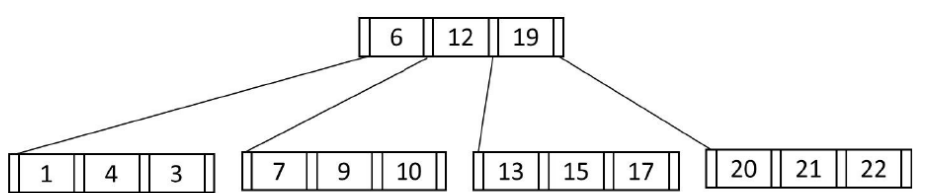
\includegraphics[width=0.7\columnwidth]{figs/q21.png}
    \end{figure}
    
    \begin{enumerate}
        \item None of the nodes will split.
        \item At least one node will split and redistribute.
        \item The total number of nodes will remain same.
        \item The height of the tree will increase.
    \end{enumerate}

    \hfill{\brak{\text{GATE CS 2025}}}

    \item Consider the $3$-way handshaking protocol for TCP connection establishment. Let the three packets exchanged during the connection establishment be denoted as P1, P2, and P3, in order. Which of the following option\brak{s} is/are TRUE with respect to TCP header flags that are set in the packets?
    \begin{enumerate}
        \item P3: SYN = 1, ACK = 1
        \item P2: SYN = 1, ACK = 1
        \item P2: SYN = 0, ACK = 1
        \item P1: SYN = 1
    \end{enumerate}

    \hfill{\brak{\text{GATE CS 2025}}}

    \item Consider the given system of linear equations for variables x and y, where k is a real-valued constant. Which of the following option\brak{s} is/are CORRECT?
    \begin{align*}
        x + ky &= 1 \\
        kx + y &= -1
    \end{align*}
    \begin{enumerate}
        \item There is exactly one value of k for which the above system of equations has no solution.
        \item There exist an infinite number of values of k for which the system of equations has no solution.
        \item There exists exactly one value of k for which the system of equations has exactly one solution.
        \item There exists exactly one value of k for which the system of equations has an infinite number of solutions.
    \end{enumerate}

    \hfill{\brak{\text{GATE CS 2025}}}

    \item Let X be a $3$-variable Boolean function that produces output as '1' when at least two of the input variables are '1'. Which of the following statement\brak{s} is/are CORRECT, where a, b, c, d, e are Boolean variables?
    \begin{enumerate}
        \item $X\brak{a,b,X\brak{c,d,e}} = X\brak{X\brak{a,b,c},d,e}$
        \item $X\brak{a,b,X\brak{a,b,c}} = X\brak{a,b,c}$
        \item $X\brak{a,b,X\brak{a,c,d}} = \brak{X\brak{a,b,a} \text{ AND } X\brak{c,d,c}}$
        \item $X\brak{a,b,c} = X\brak{a,X\brak{a,b,c},X\brak{a,c,c}}$
    \end{enumerate}

    \hfill{\brak{\text{GATE CS 2025}}}

    \item The number $-6$ can be represented as $1010$ in $4$-bit $2$'s complement representation. Which of the following is/are CORRECT $2$'s complement representation\brak{s} of $-6$?
    \begin{enumerate}
        \begin{multicols}{2}
            \item $1000\ 1010$ in $8$-bits
            \item $1111\ 1010$ in $8$-bits
            \item $1000\ 0000\ 0000\ 1010$ in $16$-bits
            \item $1111\ 1111\ 1111\ 1010$ in $16$-bits
        \end{multicols}
    \end{enumerate}

    \hfill{\brak{\text{GATE CS 2025}}}

    \item Which of the following statement\brak{s} is/are TRUE for any binary search tree \brak{BST} having n distinct integers?
    \begin{enumerate}
        \item The maximum length of a path from the root node to any other node is $\brak{n-1}$.
        \item An inorder traversal will always produce a sorted sequence of elements.
        \item Finding an element takes $O\brak{\log_2 n}$ time in the worst case.
        \item Every BST is also a Min-Heap.
    \end{enumerate}

    \hfill{\brak{\text{GATE CS 2025}}}

    \item A partial data path of a processor is given in the figure, where RA, RB, and RZ are $32$-bit registers. Which option\brak{s} is/are CORRECT related to arithmetic operations using the data path as shown?
    
    \begin{figure}[H]
        \centering
        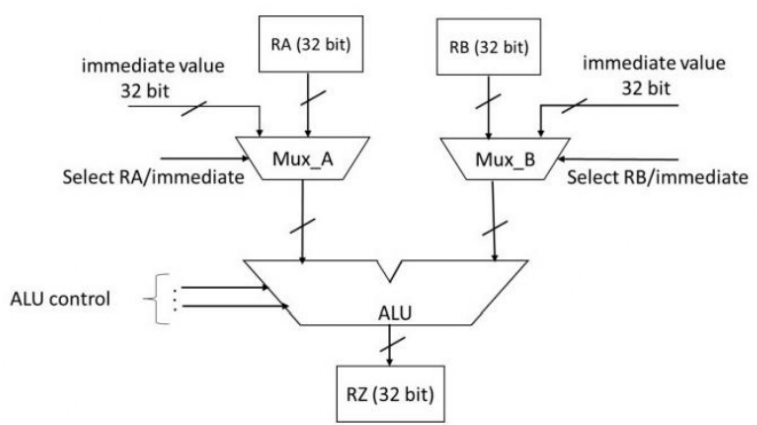
\includegraphics[width=0.8\columnwidth]{figs/q27.png}
        \label{fig:q27}
    \end{figure}
    
    \begin{enumerate}
        \item The data path can implement arithmetic operations involving two registers.
        \item The data path can implement arithmetic operations involving one register and one immediate value.
        \item The data path can implement arithmetic operations involving two immediate values.
        \item The data path can only implement arithmetic operations involving one register and one immediate value.
    \end{enumerate}

    \hfill{\brak{\text{GATE CS 2025}}}

    \item A regular language L is accepted by a non-deterministic finite automaton \brak{NFA} with n states. Which of the following statement\brak{s} is/are FALSE?
    \begin{enumerate}
        \item L may have an accepting NFA with < n states.
        \item L may have an accepting DFA with < n states.
        \item There exists a DFA with $\le 2^n$ states that accepts L.
        \item Every DFA that accepts L has $> 2^n$ states.
    \end{enumerate}

    \hfill{\brak{\text{GATE CS 2025}}}

    \item Suppose in a multiprogramming environment, the following C program segment is executed. A process goes into I/O queue whenever an I/O related operation is performed. Assume that there will always be a context switch whenever a process requests for an I/O, and also whenever the process returns from an I/O. The number of times the process will enter the ready queue during its lifetime \brak{\text{not counting the time the process enters the ready queue when it is run initially}} is \underline{\hspace{2cm}} \brak{\text{Answer in integer}}
    \begin{lstlisting}[language=C]
int main()
{
    int x=0, i=0;
    scanf("%d",&x);
    for(i=0; i<20; i++)
    {
        x=x+20;
    }
    printf("%d\n",x);
    return 0;
}
    \end{lstlisting}

    \hfill{\brak{\text{GATE CS 2025}}}

    \item Let S be the set of all ternary strings defined over the alphabet $\{a,b,c\}$. Consider all strings in S that contain at least one occurrence of two consecutive symbols, that is, "aa", "bb" or "cc". The number of such strings of length 5 that are possible is \underline{\hspace{2cm}} \brak{\text{Answer in integer}}

    \hfill{\brak{\text{GATE CS 2025}}}

    \item Consider the given function $f\brak{x}$
    \[ f\brak{x} = \begin{cases} 
          ax+b & \text{for } x < 1 \\
          x^3+x^2+1 & \text{for } x \ge 1 
       \end{cases}
    \]
    If the function is differentiable everywhere, the value of b must be \underline{\hspace{2cm}} \brak{rounded off to one decimal place}

    \hfill{\brak{\text{GATE CS 2025}}}

    \item A box contains $5$ coins: $4$ regular coins and $1$ fake coin. When a regular coin is tossed, the probability $P\brak{\text{head}}=0.5$ and for a fake coin, $P\brak{\text{head}}=1$. You pick a coin at random and toss it twice, and get two heads. The probability that the coin you have chosen is the fake coin is \underline{\hspace{2cm}} \brak{\text{rounded off to two decimal places}}

    \hfill{\brak{\text{GATE CS 2025}}}

    \item The pseudocode of a function fun \brak{} is given below:
    \begin{lstlisting}
fun (int A [0,.., n-1]){
    for i=0 to n-2
        for j=0 to n-i-2
            if (A[j] > A[j+1])
                then swap A[j] and A[j+1]
}
    \end{lstlisting}
    Let $A[0,...,29]$ be an array storing $30$ distinct integers in descending order. The number of swap operations that will be performed, if the function fun \brak{} is called with $A[0,...,29]$ as argument, is \underline{\hspace{2cm}} \brak{\text{Answer in integer}}

    \hfill{\brak{\text{GATE CS 2025}}}

    \item 
    \begin{lstlisting}[language=C]
#include <stdio.h>

void foo (int *p, int x) {
    *p = x;
}

int main() {
    int *z;
    int a = 20, b = 25;
    z = &a;
    foo (z,b);
    printf("%d",a);
    return 0;
}
    \end{lstlisting}
    The output of the given C program is \underline{\hspace{2cm}} \brak{\text{Answer in integer}}

    \hfill{\brak{\text{GATE CS 2025}}}

    \item The height of any rooted tree is defined as the maximum number of edges in the path from the root node to any leaf node.\\Suppose a Min-Heap T stores $32$ keys. The height of T is \underline{\hspace{2cm}} \brak{Answer in integer}

    \hfill{\brak{\text{GATE CS 2025}}}

    \item Consider a memory system with $1$M bytes of main memory and $16$K bytes of cache memory. Assume that the processor generates $20$-bit memory address, and the cache block size is $16$ bytes. If the cache uses direct mapping, how many bits will be required to store all the tag values? [Assume memory is byte addressable, $1K=2^{10}$, $1M=2^{20}$.]
    \begin{enumerate}
        \begin{multicols}{4}
            \item $6 \times 2^{10}$
            \item $8 \times 2^{10}$
            \item $2^{12}$
            \item $2^{14}$
        \end{multicols}
    \end{enumerate}

    \hfill{\brak{\text{GATE CS 2025}}}

    \item A processor has $64$ general-purpose registers and $50$ distinct instruction types. An instruction is encoded in $32$-bits. What is the maximum number of bits that can be used to store the immediate operand for the given instruction?
    \begin{center}
    ADD R1, \#25 \quad // R1 = R1 + 25
    \end{center}    
    \begin{enumerate}
        \begin{multicols}{4}
            \item $16$
            \item $20$
            \item $22$
            \item $24$
        \end{multicols}
    \end{enumerate}
    \hfill{\brak{\text{GATE CS 2025}}}
    \item A computer has two processors, $M_1$ and $M_2$. Four processes $P_1, P_2, P_3, P_4$ with CPU bursts of $20, 16, 25,$ and $10$ milliseconds, respectively, arrive at the same time and these are the only processes in the system. The scheduler uses non-preemptive priority scheduling, with priorities decided as follows:
    \begin{itemize}
        \item $M_1$ uses priority of execution for the processes as, $P_1 > P_3 > P_2 > P_4$ i.e., $P_1$ and $P_4$ have highest and lowest priorities, respectively.
        \item $M_2$ uses priority of execution for the processes as, $P_2 > P_3 > P_4 > P_1$ i.e., $P_2$ and $P_1$ have highest and lowest priorities, respectively.
    \end{itemize}
    A process $P_i$ is scheduled to a processor $M_k$, if the processor is free and no other process $P_j$ is waiting with higher priority. At any given point of time, a process can be allocated to any one of the free processors without violating the execution priority rules. Ignore the context switch time. What will be the average waiting time of the processes in milliseconds?
    \begin{enumerate}
        \begin{multicols}{4}
            \item $9.00$
            \item $8.75$
            \item $6.50$
            \item $7.50$
        \end{multicols}
    \end{enumerate}

    \hfill{\brak{\text{GATE CS 2025}}}

    \item Consider two relations describing teams and players in a sports league:
    \begin{itemize}
        \item teams \brak{tid, tname}: tid, tname are team-id and team-name, respectively
        \item players \brak{pid, pname, tid}: pid, pname, and tid denote player-id, player-name and the team-id of the player, respectively
    \end{itemize}
    Which ONE of the following tuple relational calculus queries returns the name of the players who play for the team having tname as 'MI'?
    \begin{enumerate}
        \item \{p.pname | p $\in$ players $\land$ \brak{$\exists$t $\in$ teams $\land$ p.tid = t.tid $\land$ t.tname = 'MI'}\}
        \item \{p.pname | p $\in$ teams $\land$ \brak{$\exists$t $\in$ players $\land$ p.tid = t.tid $\land$ t.tname = 'MI'}\}
        \item \{p.pname | p $\in$ players $\land$ \brak{$\forall$t $\in$ teams $\land$ t.tname = 'MI'}\}
        \item \{p.pname | p $\in$ teams $\land$ \brak{$\forall$t $\in$ players $\land$ t.tname = 'MI'}\}
    \end{enumerate}

    \hfill{\brak{\text{GATE CS 2025}}}

    \item A packet with the destination IP address 145.36.109.70 arrives at a router whose routing table is shown. Which interface will the packet be forwarded to?
    
    \begin{table}[H]
        \centering
        \begin{tabular}{|l|c|c|}
            \hline
            \textbf{Subnet Address} & \textbf{Subnet Mask \brak{in CIDR notation}} & \textbf{Interface} \\
            \hline
            145.36.0.0 & /16 & E1 \\
            \hline
            145.36.128.0 & /17 & E2 \\
            \hline
            145.36.64.0 & /18 & E3 \\
            \hline
            145.36.255.0 & /24 & E4 \\
            \hline
            Default & & E5 \\
            \hline
        \end{tabular}
        \caption*{}
        \label{tab:q40}
    \end{table}

    \begin{enumerate}
        \begin{multicols}{4}
            \item E3
            \item E1
            \item E2
            \item E5
        \end{multicols}
    \end{enumerate}

    \hfill{\brak{\text{GATE CS 2025}}}

    \item Let A be a $2 \times 2$ matrix as given.
    \[ A = \myvec{1 & 1 \\ 1 & -1} \]
    What are the eigenvalues of the matrix $A^{13}$?
    \begin{enumerate}
        \begin{multicols}{2}
            \item $1, -1$
            \item $2\sqrt{2}, -2\sqrt{2}$
            \item $4\sqrt{2}, -4\sqrt{2}$
            \item $64\sqrt{2}, -64\sqrt{2}$
        \end{multicols}
    \end{enumerate}

    \hfill{\brak{\text{GATE CS 2025}}}

    \item Consider the following four variable Boolean function in sum-of-product form
    \[ F\brak{b_3, b_2, b_1, b_0} = \Sigma\brak{0,2,4,8,10,11,12} \]\\where the value of the function is computed by considering $b_3 b_2 b_1 b_0$ as a $4$-bit binary number, where $b_3$ denotes the most significant bit and $b_0$ denotes the least significant bit. Note that there are no don't care terms. Which ONE of the following options is the CORRECT minimized Boolean expression for F?
    \begin{enumerate}
        \item $\overline{b_1}\overline{b_0} + \overline{b_2}\overline{b_0} + b_1\overline{b_2}b_3$
        \item $\overline{b_1}\overline{b_0} + \overline{b_2}\overline{b_0}$
        \item $\overline{b_2}\overline{b_0} + b_1 b_2 b_3$
        \item $\overline{b_0}\overline{b_2} + \overline{b_3}$
    \end{enumerate}

    \hfill{\brak{\text{GATE CS 2025}}}

    \item Let $G\brak{V,E}$ be an undirected and unweighted graph with $100$ vertices. Let $d\brak{u,v}$ denote the number of edges in a shortest path between vertices u and v in V. Let the maximum value of $d\brak{u,v}$ for u, $v \in V$ such that $u \ne v$, be $30$. Let T be any breadth-first-search tree of G. Which ONE of the given options is CORRECT for every such graph G?
    \begin{enumerate}
        \item The height of T is exactly $15$.
        \item The height of T is exactly $30$.
        \item The height of T is at least $15$.
        \item The height of T is at least $30$.
    \end{enumerate}

    \hfill{\brak{\text{GATE CS 2025}}}

    \item Consider the following two languages over the alphabet $\{a, b\}$:\\
    \begin{tabular}{ll}
    $L_1 =$& $\{\alpha\beta\alpha | \alpha \in \{a,b\}^+ \text{ AND } \beta \in \{a,b\}^+\}$\\
    $L_2 = $ & $\{\alpha\beta\alpha | \alpha \in \{a\}^+ \text{ AND } \beta \in \{a,b\}^+\}$
    \end{tabular}\\
    Which ONE of the following statements is CORRECT?
    \begin{enumerate}
        \item Both $L_1$ and $L_2$ are regular languages.
        \item $L_1$ is a regular language but $L_2$ is not a regular language.
        \item $L_1$ is not a regular language but $L_2$ is a regular language.
        \item Neither $L_1$ nor $L_2$ is a regular language.
    \end{enumerate}
    \hfill{\brak{\text{GATE CS 2025}}}
    \item Consider the following two languages over the alphabet $\{a, b, c\}$, where m and n are natural numbers.\\
    \begin{tabular}{cc}
        $L_1 =$ & $ \{a^m b^m c^{m+n} | m,n \ge 1\}$ \\
        $L_2 =$ & $\{a^m b^n c^{m+n} | m,n \ge 1\}$
    \end{tabular}\\
    Which ONE of the following statements is CORRECT?
    \begin{enumerate}
        \item Both $L_1$ and $L_2$ are context-free languages.
        \item $L_1$ is a context-free language but $L_2$ is not a context-free language.
        \item $L_1$ is not a context-free language but $L_2$ is a context-free language.
        \item Neither $L_1$ nor $L_2$ are context-free languages.
    \end{enumerate}

    \hfill{\brak{\text{GATE CS 2025}}}

    \item Which of the following statement\brak{s} is/are TRUE while computing First and Follow during top down parsing by a compiler?
    \begin{enumerate}
        \item For a production $A \rightarrow \epsilon$, $\epsilon$ will be added to First \brak{A}.
        \item If there is any input right end marker, it will be added to First\brak{S}, where S is the start symbol.
        \item For a production $A \rightarrow \epsilon$, $\epsilon$ will be added to Follow \brak{A}.
        \item If there is any input right end marker, it will be added to Follow\brak{S}, where S is the start symbol.
    \end{enumerate}

    \hfill{\brak{\text{GATE CS 2025}}}

    \item Consider a relational schema team\brak{name, city, owner}, with functional dependencies \{name $\rightarrow$ city, name $\rightarrow$ owner\}.\\The relation team is decomposed into two relations, t1\brak{name, city} and t2\brak{name, owner}. Which of the following statement\brak{s} is/are TRUE?
    \begin{enumerate}
        \item The relation team is NOT in BCNF.
        \item The relations t1 and t2 are in BCNF.
        \item The decomposition constitutes a lossless join.
        \item The relation team is NOT in 3NF.
    \end{enumerate}
    \hfill{\brak{\text{GATE CS 2025}}}
    \item Which of the following predicate logic formulae/formula is/are CORRECT representation\brak{s} of the statement: "Everyone has exactly one mother"?\\The meanings of the predicates used are:
    \begin{itemize}
        \item $mother\brak{y,x}$: y is the mother of x
        \item $noteq \brak{x, y}$: x and y are not equal
    \end{itemize}    
    \begin{enumerate}
        \item $\forall x \exists y \exists z \brak{mother\brak{y,x} \land \neg mother\brak{z,x}}$
        \item $\forall x \exists y [mother\brak{y,x} \land \forall z \brak{noteq\brak{z,y} \rightarrow \neg mother\brak{z,x}}]$
        \item $\forall x \forall y [mother\brak{y,x} \rightarrow \exists z \brak{mother\brak{z,x} \land \neg noteq\brak{z,y}}]$
        \item $\forall x \exists y [mother\brak{y,x} \land \neg \exists z \brak{noteq\brak{z,y} \land mother\brak{z,x}}]$
    \end{enumerate}

    \hfill{\brak{\text{GATE CS 2025}}}

    \item $A = \{0,1,2,3,...\}$ is the set of non-negative integers. Let F be the set of functions from A to itself. For any two functions, $f_1, f_2 \in F$, we define
    \begin{center}
        \[ \brak{f_1 \odot f_2}\brak{n} = f_1\brak{n} + f_2\brak{n} \]
    \end{center}
    for every number n in A. Which of the following is/are CORRECT about the mathematical structure $\brak{F, \odot}$
    \begin{enumerate}
        \item $\brak{F, \odot}$ is an Abelian group.
        \item $\brak{F, \odot}$ is an Abelian monoid.
        \item $\brak{F, \odot}$ is a non-Abelian group.
        \item $\brak{F, \odot}$ is a non-Abelian monoid.
    \end{enumerate}

    \hfill{\brak{\text{GATE CS 2025}}}

    \item Consider the following deterministic finite automaton \brak{DFA} defined over the alphabet, $\Sigma = \{a,b\}$. Identify which of the following language\brak{s} is/are accepted by the given DFA.
    
    \begin{figure}[H]
        \centering
        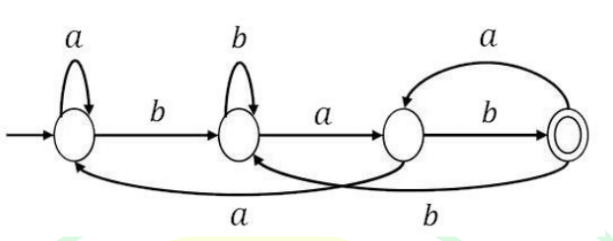
\includegraphics[width=0.6\columnwidth]{figs/q50.png}
        \caption*{}
        \label{fig:q50}
    \end{figure}
    
    \begin{enumerate}
        \item The set of all strings containing an even number of b's.
        \item The set of all strings containing the pattern bab.
        \item The set of all strings ending with the pattern bab.
        \item The set of all strings not containing the pattern aba.
    \end{enumerate}

    \hfill{\brak{\text{GATE CS 2025}}}

    \item A disk of size $512$M bytes is divided into blocks of $64$K bytes. A file is stored in the disk using linked allocation. In linked allocation, each data block reserves $4$ bytes to store the pointer to the next data block. The link part of the last data block contains a NULL pointer \brak{also of 4 bytes}. Suppose a file of $1$M bytes needs to be stored in the disk. Assume, $1K=2^{10}$ and $1M=2^{20}$. The amount of space in bytes that will be wasted due to internal fragmentation is \underline{\hspace{2cm}} \brak{\text{Answer in integer}}

    \hfill{\brak{\text{GATE CS 2025}}}

    \item Refer to the given 3-address code sequence. This code sequence is split into basic blocks. The number of basic blocks is \underline{\hspace{2cm}} \brak{\text{Answer in integer}}
    
    \begin{lstlisting}
1001: i = 1
1002: j = 1
1003: t1 = 10 * i
1004: t2 = t1 + j
1005: t3 = 8 * t2
1006: t4 = t3 - 88
1007: a[t4] = 0.0
1008: j = j + 1
1009: if j <= 10 goto 1003
1010: i = i + 1
1011: if i <= 10 goto 1002
1012: i = 1
1013: t5 = i - 1
1014: t6 = 88 * t5
1015: a[t6] = 1.0
1016: i = i + 1
1017: if i <= 10 goto 1013
    \end{lstlisting}
    \hfill{\brak{\text{GATE CS 2025}}}
    \item A computer has a memory hierarchy consisting of two-level cache \brak{L1 and L2} and a main memory. If the processor needs to access data from memory, it first looks into L1 cache. If the data is not found in L1 cache, it goes to L2 cache. If it fails to get the data from L2 cache, it goes to main memory, where the data is definitely available. Hit rates and access times of various memory units are shown in the figure. The average memory access time in nanoseconds \brak{ns} is \underline{\hspace{2cm}}. \brak{\text{rounded off to two decimal places}}
    \begin{figure}[H]
        \centering
        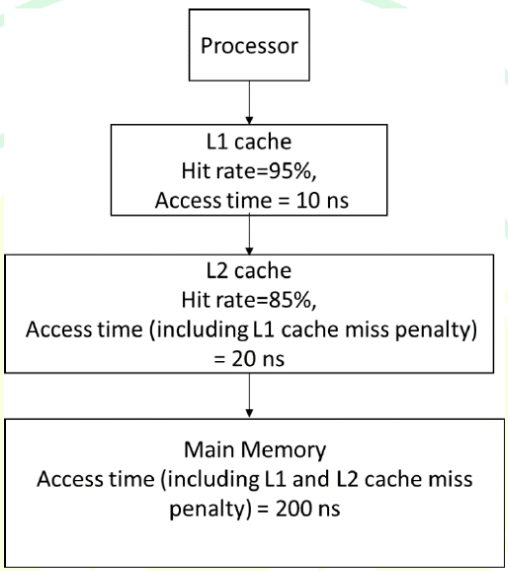
\includegraphics[width=0.5\columnwidth]{figs/q53.png}
        \label{fig:q53}
    \end{figure}

    \hfill{\brak{\text{GATE CS 2025}}}

    \item In optimal page replacement algorithm, information about all future page references is available to the operating system \brak{OS}. A modification of the optimal page replacement algorithm is as follows:\\The OS correctly predicts only up to next $4$ page references \brak{including the current page} at the time of allocating a frame to a page.\\A process accesses the pages in the following order of page numbers:
    \begin{center}
    $1, 3, 2, 4, 2, 3, 1, 2, 4, 3, 1, 4$.
    \end{center}
    If the system has three memory frames that are initially empty, the number of page faults that will occur during execution of the process is \underline{\hspace{2cm}} \brak{\text{Answer in integer}}

    \hfill{\brak{\text{GATE CS 2025}}}

    \item Consider the following database tables of a sports league.\\
    \begin{tabular}{ll}
        player \brak{pid, pname, age} & team \brak{tid, tname, city, cid} \\
        coach \brak{cid, cname} & members \brak{pid, tid}
    \end{tabular}\\
    An instance of the table and an SQL query are given.
    \begin{figure}[H]
        \centering
        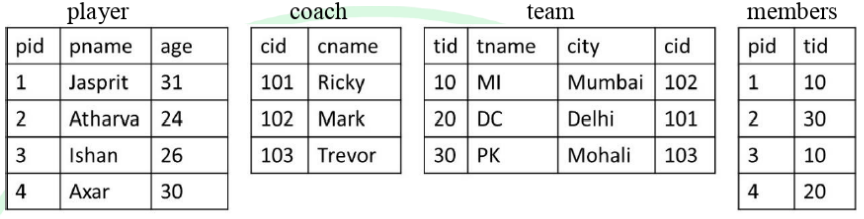
\includegraphics[width=\columnwidth]{figs/q55.png}
    \end{figure}
    
    \begin{lstlisting}[language=SQL]
SELECT MIN (P.age)
FROM player P
WHERE P.pid IN (
    SELECT M.pid
    FROM team T, coach C, members M
    WHERE C.cname = 'Mark'
    AND T.cid = C.cid
    AND M.tid = T.tid
)
    \end{lstlisting}
    
    The value returned by the given SQL query is \underline{\hspace{2cm}} \brak{\text{Answer in integer}}

    \hfill{\brak{\text{GATE CS 2025}}}

    \item Suppose a $5$-bit message is transmitted from a source to a destination through a noisy channel. The probability that a bit of the message gets flipped during transmission is $0.01$. Flipping of each bit is independent of one another. The probability that the message is delivered error-free to the destination is \underline{\hspace{2cm}} \brak{\text{rounded off to three decimal places}}

    \hfill{\brak{\text{GATE CS 2025}}}

    \item Suppose a message of size $15000$ bytes is transmitted from a source to a destination using IPv4 protocol via two routers as shown in the figure. Each router has a defined maximum transmission unit \brak{MTU} as shown in the figure, including IP header. The number of fragments that will be delivered to the destination is \underline{\hspace{2cm}}. \brak{Answer in integer}
    \begin{figure}[H]
        \centering
        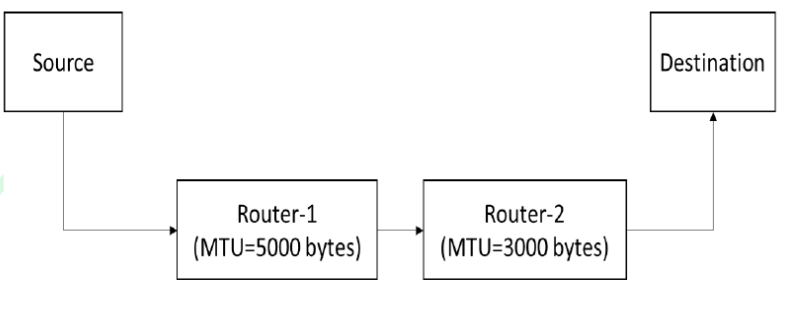
\includegraphics[width=0.7\columnwidth]{figs/q57.png}
    \end{figure}

    \hfill{\brak{\text{GATE CS 2025}}}

    \item Consider a probability distribution given by the density function $P\brak{x}$.
    \[ P\brak{x} = \begin{cases} 
          Cx^2, & \text{for } 1 \le x \le 4 \\
          0, & \text{for } x < 1 \text{ or } x > 4
       \end{cases}
    \]
    The probability that x lies between 2 and 3, i.e., $P\brak{2 \le x \le 3}$ is \underline{\hspace{2cm}} \brak{\text{rounded off to three decimal places}}

    \hfill{\brak{\text{GATE CS 2025}}}

    \item Consider a finite state machine \brak{FSM} with one input X and one output f, represented by the given state transition table. The minimum number of states required to realize this FSM is \underline{\hspace{2cm}}. \brak{Answer in integer}
    
    \begin{table}[H]
        \centering
        \begin{tabular}{|c|c|c|c|c|}
            \hline
            \textbf{Present state} & \multicolumn{2}{c|}{\textbf{Next state}} & \multicolumn{2}{c|}{\textbf{Output f}} \\
            \cline{2-5}
             & \textbf{X=0} & \textbf{X=1} & \textbf{X=0} & \textbf{X=1} \\
            \hline
            A & F & B & 0 & 0 \\
            \hline
            B & D & C & 0 & 0 \\
            \hline
            C & F & E & 0 & 0 \\
            \hline
            D & A & G & 0 & 1 \\
            \hline
            E & D & C & 0 & 0 \\
            \hline
            F & F & B & 1 & 1 \\
            \hline
            G & G & H & 1 & 0 \\
            \hline
            H & A & G & 1 & 0 \\
            \hline
        \end{tabular}
        \caption*{}
    \end{table}

    \hfill{\brak{\text{GATE CS 2025}}}

    \item Consider the given sequential circuit designed using D-Flip-flops. The circuit is initialized with some value \brak{initial state}. The number of distinct states the circuit will go through before returning back to the initial state is \underline{\hspace{2cm}}. \brak{\text{Answer in integer}}
    \begin{figure}[H]
        \centering
        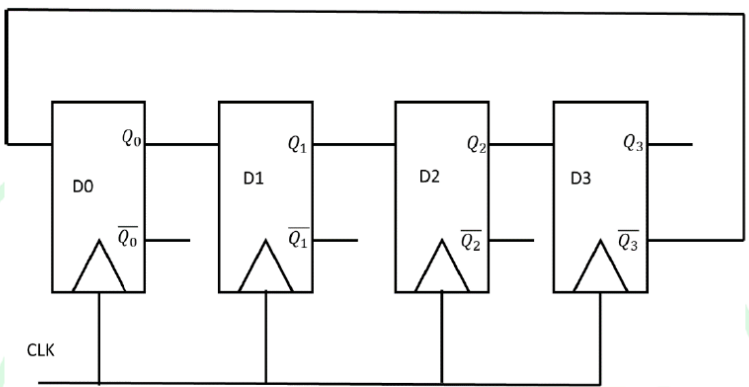
\includegraphics[width=0.7\columnwidth]{figs/q60.png}
    \end{figure}

    \hfill{\brak{\text{GATE CS 2025}}}

    \item
    \begin{lstlisting}[language=C]
#include <stdio.h>

int foo (int S[], int size) {
    if (size == 0) return 0;
    if (size == 1) return 1;
    if (S[0] != S[1]) return 1 + foo(S + 1, size - 1);
    return foo(S + 1, size - 1);
}

int main() {
    int A[] = {0,1,2,2,2,0,0,1,1};
    printf("%d", foo(A,9));
    return 0;
}
    \end{lstlisting}
    The value printed by the given C program is \underline{\hspace{2cm}}. \brak{\text{Answer in integer}}

    \hfill{\brak{\text{GATE CS 2025}}}

    \item Let LIST be a datatype for an implementation of linked list defined as follows:
    \begin{lstlisting}[language=C]
typedef struct list {
    int data;
    struct list *next;
} LIST;
    \end{lstlisting}
    Suppose a program has created two linked lists, L1 and L2, whose contents are given in the figure below \brak{code for creating L1 and L2 is not provided here}. L1 contains 9 nodes, and L2 contains 7 nodes.
    
    Consider the following C program segment that modifies the list L1. The number of nodes that will be there in L1 after the execution of the code segment is \underline{\hspace{2cm}}. \brak{\text{Answer in integer}}
    
    \begin{figure}[H]
        \centering
        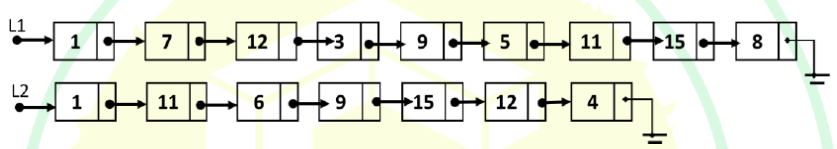
\includegraphics[width=\columnwidth]{figs/q62.png}
    \end{figure}
    
    \begin{lstlisting}[language=C]
int find (int query, LIST *list) {
    while (list != NULL) {
        if (list->data == query) return 1;
        list = list->next;
    }
    return 0;
}

int main () {
    ptr1 = L1;
    while (ptr1->next != NULL) {
        query = ptr1->next->data;
        if (find(query, L2))
            ptr1->next = ptr1->next->next;
        else
            ptr1 = ptr1->next;
    }
    return 0;
}
    \end{lstlisting}

    \hfill{\brak{\text{GATE CS 2025}}}

    \item Consider the following C program:
    \begin{lstlisting}[language=C]
#include <stdio.h>

int gate (int n) {
    int d, t, newnum, turn;
    newnum = turn = 0;
    t = 1;
    while (n >= t) t *= 10;
    t /= 10;
    while (t > 0) {
        d = n / t;
        n = n % t;
        t /= 10;
        if (turn) newnum = 10 * newnum + d;
        turn = (turn + 1) % 2;
    }
    return newnum;
}

int main () {
    printf ("%d", gate (14362));
    return 0;
}
    \end{lstlisting}
    The value printed by the given C program is \underline{\hspace{2cm}}. \brak{Answer in integer}

    \hfill{\brak{\text{GATE CS 2025}}}

    \item The maximum value of x such that the edge between the nodes B and C is included in every minimum spanning tree of the given graph is \underline{\hspace{2cm}}. \brak{\text{answer in integer}}
    
    \begin{figure}[H]
        \centering
        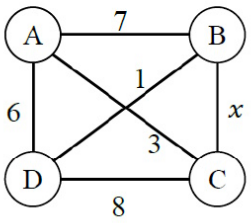
\includegraphics[width=0.5\columnwidth]{figs/q64.png}
    \end{figure}

    \hfill{\brak{\text{GATE CS 2025}}}

    \item In a double hashing scheme, $h_1\brak{k} = k \text{ mod } 11$ and $h_2\brak{k} = 1 + \brak{k \text{ mod } 7}$ are the auxiliary hash functions. The size m of the hash table is $11$. The hash function for the i-th probe in the open address table is $[h_1\brak{k} + i h_2\brak{k}] \text{ mod } m$. The following keys are inserted in the given order: $63, 50, 25, 79, 67, 24$.\\The slot at which key $24$ gets stored is \underline{\hspace{2cm}}. \brak{\text{Answer in integer}}
    \hfill{\brak{\text{GATE CS 2025}}}

\end{enumerate}
\end{document}
